\documentclass[12pt, twoside]{article}

% Erlaube einfaches copy & paste aus der generierten pdf
\usepackage[T1]{fontenc}
% Erlaube überall underscore zu benutzen ohne \_ schreiben zu müssen
% https://tex.stackexchange.com/questions/20890/define-an-escape-underscore-environment 
\catcode`\_=12
\usepackage[utf8]{inputenc}

% Deutsche Bezeichnungen wie etwa "Inhaltsverzeichnis", statt "Contents"
\usepackage[german]{babel}

% Deutsche Absätze
\parindent 0pt

% Dieses Package ermöglich einfügen von Bildern mittels \includegraphics
\usepackage{graphicx}

% Zwinge Latex zum einfügen von bildern dort wo man sie im tex 
% Dokument hinterlegt mittels \begin{figure}[H]   
\usepackage{float}

% Ändere Highlight Color
\usepackage{color}
\definecolor{insertedCode}{RGB}{190, 230, 190} 

% Syntax Highlighting 
\usepackage{minted}
% Lösche rote Rahmen in minted Quelltext und nutze das Visual Studio Theme
\usemintedstyle{vs}
\setminted{autogobble=true, fontsize=\footnotesize, baselinestretch=1.0, frame=lines, mathescape, linenos, numbersep=5pt, framesep=2mm, breaklines, highlightcolor=insertedCode, breakafter=_@|.}
\renewcommand{\listingscaption}{Code Snippet}
% Veringere Abstand zum Untertitel
\AtEndEnvironment{listing}{\vspace{-14pt}} % <-
% Bei Syntaxfehler keine roten vierecke darum zeichnen
% https://tex.stackexchange.com/questions/343494/minted-red-box-around-greek-characters 


\usepackage{etoolbox}

\makeatletter
\AtBeginEnvironment{minted}{\dontdofcolorbox}
\def\dontdofcolorbox{\renewcommand\fcolorbox[4][]{##4}}
\makeatother



\usepackage[autostyle,german=quotes]{csquotes}

% Für Hintergrundbilder mittels \AddToShipoutPicture
\usepackage{eso-pic}

% Bilder transparent machen
\usepackage{transparent}

% Fallunterscheidungen wie etwa gerade und ungerade Seiten
\usepackage{ifthen}

% Einfügen von Tabellen
\usepackage{tabularx}

% Literaturverzeichnisse verwenden
% backref=true - referenziert von Literaturverzeichnis zurück auf die Seite wo zitiert wurde
\usepackage[style=authortitle, natbib, backend=biber, backref=true]{biblatex}
% Nummer der Zitation nicht hochgestellt, sondern sondern mit
% normaler Textgröße und einem Punkt nach der Nummer
% Beispiel: 1. Teller,”Visibility computations in densely occluded polyhedral environments.“, S. 19
\makeatletter% 
\long\def\@makefntext#1{% 
  \parindent 1em\noindent \hb@xt@ 1.8em{\hss  \hbox {{\normalfont \@thefnmark }}. }#1}%
\makeatother

% Texte für die zurückreferenzierung definieren
\DefineBibliographyStrings{german}{%
  backrefpage = {Zitiert auf der Seite},% originally "cited on page"
  backrefpages = {Zitiert auf den Seiten},% originally "cited on pages"
}

% Links mit Sprungmarken
\usepackage{hyperref}
\hypersetup{
  colorlinks=true,
  linkcolor=black, % Setz die Farbe von Links im 
                   % Inhaltsverzeichnis zurück auf schwarz
  citecolor=black, % Farbe von Literaturlinks = schwarz
  urlcolor=blue    % Farbe von URLs = blau     
}


% Referezieren von Kapiteln mit ihrem Titel
\usepackage{nameref}

% Einfügen von PDFs
\usepackage{pdfpages} 

% Seitenränder
\usepackage{geometry}
\geometry{a4paper, top=20mm, left=40mm, right=20mm, bottom=20mm, headsep=12mm, footskip=12mm}

% Absatzformat
\parskip2ex		% Absatzabsstand	
\parindent0ex		% Absatzeinzug

% Package zum hinzufügen eines Glossars
\usepackage{glossaries}  
\setacronymstyle{long-short}  
\newacronym{eler}{ELER}{Europäischer Landwirtschaftsfond für die Entwicklung des ländlichen Raum}  

% Auf gleiche footnote erneut verweisen mit cleveref
% Achtung: Wenn cleveref nicht zum ende geladen wird gibt es evtl. die Fehlermeldung: Package cleveref Error: cleveref must be loaded after amsmath!.
\usepackage{cleveref}
% Auf erneut verweisen
\crefformat{footnote}{#2\footnotemark[#1]#3} 

% Abbildungsunterschrift anpassen
% https://tex.stackexchange.com/questions/86120/font-size-of-figure-caption-header/86121
\usepackage[font=footnotesize,labelfont=bf]{caption}
% Abstand anpassen
% https://tex.stackexchange.com/questions/45990/how-can-i-modify-vertical-space-between-figure-and-caption
\setlength{\abovecaptionskip}{10pt plus 3pt minus 2pt} 

% Nutze unterschiedliche fußnoten (1,2,3 und a,b,c)
\usepackage[para]{manyfoot}
% \footnoteL{https://google.com}
\DeclareNewFootnote{L}[Roman]
% \footnoteI{https://google.com}
\DeclareNewFootnote{I}[alph]

% fußnoten nacheinander mit Kommas
% \footnote{Einz}\footnote{Zwei}
\usepackage[multiple]{footmisc}
 

\addbibresource{literatur/literatur.bib}

\begin{document}
 

\begin{center}
    

    %\includegraphics[width=0.5\paperwidth]{img/logo/hs_harz_logo.png}

    \vspace{20mm}

    \Huge
    \textsc{Flutter vs Complexity}

    \vspace{5mm}

    \Large
    \textsc{Eine Eallstudie zur Lösung einer komplexen Problemstellung mit Hilfe einer Reihe an Softwaretechnischer Hilfsmittel mit Flutter}
    \vfill
    
    % https://pascalhertleif.de/artikel/richtlinien-fur-fallstudien-in-der-software-entwicklung/

    \normalsize
    Vorgelegt von:

    \textbf{Alexander Johr}

    Meine Adresse

    \vspace{20mm}

    \begin{tabular}{r c}
        Erstprüfer: & Prof. Jürgen Singer Ph.D. \\
        Zweitprüfer: & Prof. Daniel Ackermann \\
        Datum: & 02.11.2020 \\
    \end{tabular}

    \vspace{5mm}

\end{center}


  
\newpage\null\thispagestyle{empty}\newpage

\newpage
\thispagestyle{empty}

Hochschule Harz\newline
Fachbereich Automatisierung und Informatik
\vfill
\begin{center}

\large{\textsc{Thema und Aufgabenstellung der Masterarbeit}}

\large{\textsc{MA AI 29/2021}}

\vfill

\large{\textsc{für Herrn Alexander Johr}}

\vfill

%\vfill
\Large{\textsc{Entwicklung einer Formularanwendung mit Kompatibilitätsvalidierung der Einfach- und Mehrfachauswahl-Eingabefelder}}



\end{center}

\vfill

%gut darlegen könnendie methode spielt mehr die rolle


%andeuten nicht ins detail

%ich möchte mich testing


%kern des themas

%immer zurück kommen

%höhere eigen zum ergebis

%das liebesleben der tennisbällen unter einfluss des mondscheins

%größtmögliche unfall der passiert mal wahrscheinlichkeit 

%kompliziertheit komplexität

%werner von braun
%triebwerke geschrottet

%doku 
%arte 3 sat
%allgemein menschheit in den weltraum

%feindifferenziert


%Frage an Herr Ackermann / Singer: Vergleich mit Angular Dart, Angular allgemein, XAML WPF, evtl. etwas 

%Aber nicht alle

%Deshalb Fallstudie, richtig?

Das Thünen-Institut für Ländliche Räume wertet Daten zu Maßnahmen auf landwirtschaftlich genutzten Flächen aus. Dafür müssen entsprechende Maßnahmen
bundesweit mit Zeitbezug auswertbar sein und mit Attributen versehen werden.
Um die Eingabe für die Wissenschaftler des Instituts zu beschleunigen
 und um fehlerhafte Eingaben zu minimieren, soll eine 
 spezielle Formularanwendung entwickelt werden.
Neben herkömmlichen Freitextfeldern beinhaltet das gewünschte Formular zum Großteil Eingabefelder für Einfach- und Mehrfachauswahl.
Je nach Feld kann die Anzahl der Auswahloptionen mitunter zahlreich sein.
Dem Nutzer sollen daher nur solche Auswahloptionen angeboten werden,
die zusammen mit der zuvor getroffenen Auswahl sinnvoll sind.

\vspace{14pt}

Im Wesentlichen ergibt sich die Kompatibilität 
der Auswahloptionen aus der Bedingung, 
dass für dasselbe oder ein anderes Eingabefeld eine Auswahlmöglichkeit gewählt bzw.
nicht gewählt wurde. Diese Bedingungen müssen durch 
Konjunktion und Disjunktion verknüpft werden können.
In Sonderfällen muss ein Formularfeld jedoch auch 
die Konfiguration einer vom Standard abweichenden Bedingung
ermöglichen. 
Wird dennoch versucht,
eine deaktivierte Option zu selektieren, wäre eine Anzeige der
inkompatiblen sowie der stattdessen notwendigen Auswahl ideal.

\vspace{14pt}
Die primäre Zielplattform der Anwendung ist das Desktop-Betriebssystem
Microsoft Windows 10.
Idealerweise ist die Formularanwendung auch auf weiteren Desktop-Plattformen sowie
mobilen Endgeräten wie Android- und iOS-Smartphones und -Tablets
lauffähig. Die Serialisierung der eingegebenen Daten genügt dem Institut 
zunächst als Ablage einer lokalen Datei im JSON-Format. 
%Nach der Testphase des Eingabeformulars erfolgt der Import der Daten in das Relationale Datenbank-Management System ProstgreSQL. 

% Beim Versuch, eine inkompatible Auswahl zu selektieren,
% könnte die Visualisierung eines Mengendiagramms der erforderlichen und invaliden
% Auswahlfelder und die User Experience weiter verbessern.
% Als Ergebnis der Anforderungsanalyse wurde 
% ein UI-Framework ausgewählt,
% welches neben weiteren Auswahlkriterien 
% insbesondere ein hohes Maß an Flexibilität erlaubt: Flutter.





%Die freiheiten in der Oberflächenentwicklung 


%Ziel dieser Masterarbeit ist die Entwicklung der Formular-Anwendung 
%und dabei den Entwicklungsschitteprozess und die 

%Flutter bietet arbeitet mit funktionaler UI. Damit gibt Flutter die Wahl des Zustandsmanagements.


%Dies bietet einige Vorlteile. Koontrolle über die Performance.
%Vereinfachte Fehlersuche in der UI. Freiheiten in der Entwicklung der UI.
%Konfiguration von wiederverwendbaren Oberflächenkomponenten mithilfe des Strategy Entwurfsmusters.
%Doch es ergeben sich auch Nachteile: 
%Es gibt keine goto Methode für zustandsmanagement sondern eine Auswahl der 
%richtigen Methoe muss auf Grundlage der Anfforderungen gewählt werden.

%Zier der Arbeit ist es die Vorteile und Nachteile näher zubeleuchten.
%Dies soll mit der Entwicklung einer Anwendung in Flutter begleitet werden. Die Anwendung soll eine komplexes Eingabe-Formular für das Thünen institut in Braunschweig sein.



%Templates <-> Functional UI

%Exceptions <-> Hot Reload

%Stragety Pattern

%Reguläre ausdrücke

%Refactoring

%Programmgenerierung JSON AOT vs C\# Reflection


%Kontrolle

%Nachteile

%Provider BloC <-> Provider
%Eine  Data Binding

%Die zwei b Die beiden 

%Performance

%Die Produkte QlikView und Qlik Sense - Business Intelligence Software des Software\-unter\-nehmens Qlik - bieten ihren Anwendern mit einer Reihe an unterschiedlichen Diagramm\-typen einen Überblick über ihre Geschäftsdaten mittels Ad-hoc-Analysen. Nicht alle Wünsche der Anwender lassen sich über die Konfigurations\-möglich\-keiten dieser vorgefertigten Diagramme abdecken. Eine Alternative stellen die sogenannten Extension Objects und Document Extensions dar, die mit mithilfe von Webtechnologien wie JavaScript, HTML, CSS und XML entwickelt werden können. Die Entwicklung von Programmen mit JavaScript erweist sich jedoch gegenüber der Entwicklung mit anderen Programmiersprachen als sehr mühsam.


%Ziel dieser Bachelorarbeit ist es die Entwicklung dieser Extension Objects sowie Document Extensions mit der Programmiersprache Dart von Google umzusetzen, da sich diese für die Entwicklung skalierbarer und strukturierter Webanwendungen eignet. Die Arbeit bietet einen Leitfaden wie solche Extensions mit Dart entwickelt werden können und welche Vor- und Nachteile dies gegenüber der Entwicklung mit JavaScript bietet. 


%Die Bachelorarbeit beinhaltet folgende Teilaufgaben:
%\begin{itemize}
%	\itemsep0em
%	\item Analyse der Unterschiede von QlikView 11 und Qlik Sense bei der Entwicklung von Extension Objects sowie von Document Extensions
%	\item Analyse der Einschränkungen von Extensions Objects gegenüber der von QlikView 11 und Qlik Sense mitgelieferten Sheet Objects
%	\item Analyse der Auswirkungen der Extensions auf die Performance
%	\item Analyse der Vor- und Nachteile der Entwicklung von Extensions mit Dart im Vergleich zur Entwicklung von Extensions mit JavaScript
%	\item Entwicklung von zeitsparenden Methoden zur Entwicklung von Extensions
%	\item Bewertung der Ergebnisse
%\end{itemize}

\vspace{14pt}
Die Masterarbeit umfasst folgende Teilaufgaben:
\begin{itemize}
    \itemsep0em
\item Analyse der Anforderungen an die Formularanwendung
\item Evaluation der angemessenen Technologie für die Implementierung
\item Entwurf und Umsetzung der Übersichts- und Eingabeoberfläche
\item Konzeption und Implementierung der Validierung der Eingabefelder
\item Entwicklung von automatisierten Testfällen zur Qualitätskontrolle
\item Bewertung der Implementierung und Vergleich mit den Wunschkriterien
\end{itemize}


%Die Freiheiten der Oberflächenentwicklung in Flutter sollen genutzt werden, um 
%visuellen Komponenten zu erstellen, die durch Einsatz des Strategie-Entwurfsmusters
%im hohen Maße anpassbar sind.



%Da die Aktualisierung von Flutter-Views nicht automatisch erfolgt, muss ein angemessenes 
%Zustandsmanagement evaluiert und eingesetzt werden.
%Eine angemessene Technologie zur Serialisierung soll gewählt und 
%das Persistieren der eingegebenen Datensätze damit umgesetzt werden.
%Durch die Menge der Auswahlfelder ist bei Weiterentwicklung der APIs mit 
%hohem Migrationsaufwand der Codebasis zu rechnen. Der Einsatz von regulären Ausdrücken
%soll helfen, den Prozess zu automatisieren. Die Entwicklung automatisierter Testfälle
%soll weiterhin ermöglichen, Fehler bei der Weiterentwicklung zeitnah zu erkennen.



%Die Masterarbeit beinhaltet damit folgende Teilaufgaben:
%\begin{itemize}
%	\itemsep0em
%	\item Evaluation des Zustandsmanagements und Implementierung des View Models
%    \item Entwicklung von wiederverwendbarer Komponenten des Views und Anpassung dieser mit dem Strategie Entwurfsmuster
%    \item Auswahl der Technologie zur Serialisierung und Implementierung der Persistierung des Models
%	\item Migration der Codebasis auf aktualisierte APIs mittels Regulärer Ausdrücke
%	\item Entwicklung von Automatisierten Testfällen
%\end{itemize}

\vfill
\vfill
\vfill 
\vfill
\vfill

\begin{tabularx}{\textwidth}{@{} *2{>{\centering\arraybackslash}X}@{}}
Prof. Jürgen Singer Ph.D. & Prof. Daniel Ackermann \\
1. Prüfer                 & 2. Prüfer	 \\
\end{tabularx}	     

   

Inhaltsverzeichnis 
\listoffigures 
%List of Listings umbenennen
\renewcommand{\listoflistingscaption}{Listingsverzeichnis}

%Listingsverzeichnis
\addcontentsline{toc}{section}{Listingsverzeichnis}
\listoflistings

\section{Anforderungen}

Dieses Kapitel behandelt die Anforderungen

\begin{itemize}
    \item Performance: Hohe Anzahl Eingabefelder
    \item nested formulars
\end{itemize}



\section{Technologie Auswahl}

Dieses Kapitel behandelt die Auswahl der Frontend-Technologie für die Umsetzung der Formular-Anwendung. Dazu  werden im ersten Schritt die dafür in Frage kommende Technologien identifiziert.  Anschließend wird der Trend der Popularität dieser Technologien miteinander verglichen. Die daraus resultierenden Kandidaten sollen dann  detaillierter untersucht werden. In Hinblick auf die Anforderungen an die Formular-Anwendung soll dabei die angemessenste Frontend-Technologie ausgewählt werden.



\subsection{Trendanalyse}

Zwei Quellen wurden für die Analyse der Technologie-Trends ausgewählt: die Ergebnisse der jährlichen Stack Overflow Umfragen und das Such-Interesse von Google Trends. 

\paragraph{Stack Overflow Umfrage}
Die Internet-Plattform Stack Overflow richtet sich an Softwareentwickler und bietet ihren Nutzern die Möglichkeiten, Fragen zu stellen, Antworten einzustellen und Antworten anderer Nutzer auf- und abzuwerten. 
Besonders für Fehlermeldungen, die häufig während der Softwareentwicklung auftreten, findet man auf dieser Plattform rasch die Erklärung und den Lösungsvorschlag gleich mit. Dadurch lässt sich auch die Herkunft des Domain-Namens herleiten:

\begin{quotation}
We named it Stack Overflow, after a common type of bug that causes software to crash -- plus, the domain name stackoverflow.com happened to be available. - Joel Spolsky, Mitgründer von Stack Overflow \footnote{\cite{TheUnprovenPath}}
\end{quotation}

Aufgrund des Erfolgsrezepts von Stack Overflow ist die Plattform kaum einem Softwareentwickler unbekannt. Dementsprechend nehmen auch jährlich tausende Entwickler an den von Stack Overflow herausgegebenen Umfragen teil. Seit  2013 beinhalten die Umfragen auch die Angabe der aktuell genutzten und in Zukunft gewünschten Frontend-Technologien.
Stackoverflow erstellt aus diesen gesammelten Daten Auswertungen und Übersichten. Doch gleichzeitig werden die zugrundeliegenden Daten veröffentlicht. \footnote{\cite{StackOverflowInsights}} 

Um den Trend der Beliebtheit der Frontend-Technologien aufzuzeigen, wurde ein Jupyter Notebook erstellt. Es transformiert die Daten in ein einheitliches Format, da die  Umfrageergebnisse von Jahr zu Jahr in einer unterschiedlichen Struktur abgelegt wurden. Anschließend erstellt es Diagramme, die im Folgenden analysiert werden. Das Jupyter Notebook ist im  Anhang zu finden.

\paragraph{Google Trends} Suchanfragen die an die Suchmaschine Google  abgesetzt werden, lassen sich  über den Dienst Google Trends  als Trenddiagramm Visualisieren. Um das relative Such-Interesse abzubilden, werden die Ergebnisse normalisiert, um die Ergebnisse auf einer Skala von 0 bis 100 darstellen zu können. \footnote{Vgl. \cite{GoogleTrendsHilfe}}

\begin{quotation}
Google Trends ist keine wissenschaftliche Umfrage und sollte nicht mit Umfragedaten verwechselt werden. Es spiegelt lediglich das Suchinteresse an bestimmten Themen wider. \footnote{\cite{GoogleTrendsHilfe}}
\end{quotation}

Genau aus diesem Grund wird Google Trends im Folgenden lediglich zum Abgleich der Ergebnisse der Stack Overflow Umfrage eingesetzt. 

\subsubsection{Frameworks mit geringer Relevanz}

NativeScript, Sencha (bzw. Sencha Touch) und Appcelerator spielen in den Umfrageergebnisse eine Untergeordnete Rolle. Dies ist in den aufsummierten Stimmen von 2013 bis 2020 für alle in der Umfrage auftauchenden Frontend-Technologien zu sehen (Abb. \ref{fig:SummeDerStimmen}).

\begin{figure}[h]
	\centering
    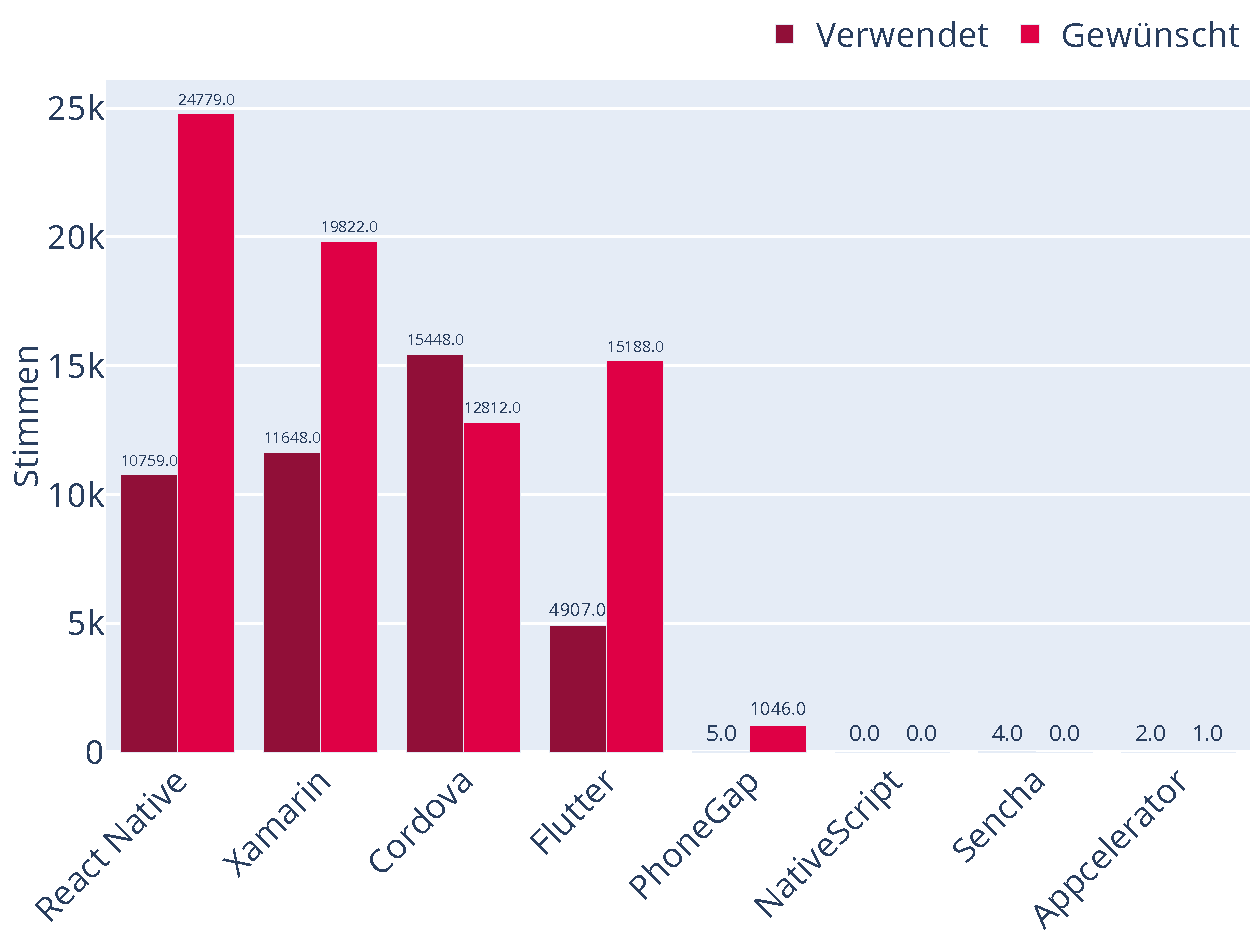
\includegraphics[width=1.0\textwidth]{Charts/Stack Overflow Umfrage/Summe der Stimmen.pdf}
	\caption[Stimmen der Stack Overflow Umfrage von 2013 bis 2020]{Summe der Stimmen der Stack Overflow Umfrage von 2013 bis 2020, Quelle: Eigene Abbildung, Notebook: Charts/Stack Overflow Umfrage/Stack Overflow Umfrage.ipynb}
	\label{fig:SummeDerStimmen}
\end{figure}

Auch das Suchinteresse auf Google ist für diese Frameworks äußerst gering. In Abbildung \ref{fig:SuchinteresseGeringeRelevanz} werden NativeScript, Sencha, Appcelerator und auch Adobe PhoneGap mit Apache Cordova für das relative Suchinteresse verglichen. 

\begin{figure}[h]
	\centering
    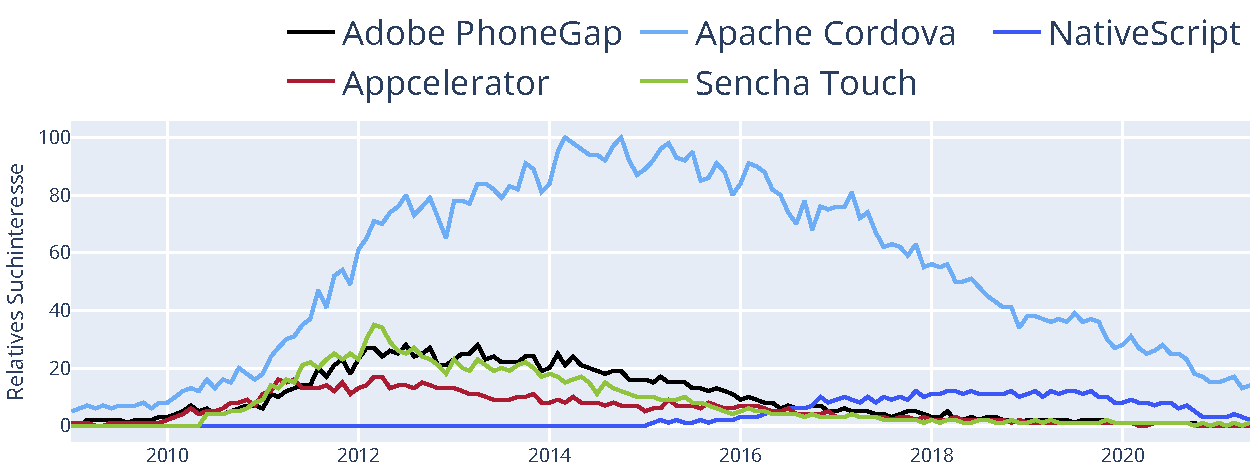
\includegraphics[width=1.0\textwidth]{Charts/Google Trends/Suchinteresse geringe Relevanz.pdf}
	\caption[]{, Quelle: Eigene Abbildung, Notebook: Charts/Google Trends/Google Trends.ipynb, Daten-Quelle: Google Trends\footnote{\cite{FaqPhoneGapDocs}}}
	\label{fig:SuchinteresseGeringeRelevanz}
\end{figure}


\paragraph{Verwandte Technologien zu Apache Cordova} Das Ionic Framework taucht in den Ergebnissen der Stack Overflow Umfragen nicht auf. Ein Grund dafür könnte sein, dass es auf Apache Cordova aufbaut\footnote{\cite{TheLastWordOnCordovaAndPhoneGap}}, welches bereits in den Ergebnissen vorkommt. Adobe PhoneGap taucht zwar in den Ergebnissen von 2013 mit 1043 Stimmen auf (Siehe Abbildung \ref{fig:CordovaUndPhoneGapStimmen}), verliert jedoch in den Folgejahren mit weniger als 10 Stimmen abrubt an Relevanz.  Das stimmt nicht mit dem Suchinteresse auf Google überein, da es dort ab 2013 sogar steigt, wie in Abbildung \ref{fig:SuchinteresseGeringeRelevanz} zu sehen ist. 2013 existierte PhoneGap noch als extra Mehrfachauswahlfeld in den Daten, während es ab 2014 nur noch in dem Feld für die sonstigen Freitext Angaben auftaucht \footnote{Vgl. \cite{StackOverflowInsights}}. Auch Adobe PhoneGap baut auf Apache Cordova auf\footnote{Vgl. \cite{FaqPhoneGapDocs}}. Für diese Auswertung spielen diese verwandten Technologien eine untergeordnete Rolle, da sie auch in den Google Trends weit hinter Apache Cordova zurückbleiben (Abb. \ref{fig:SuchinteresseGeringeRelevanz}).
 
\begin{figure}[h]
	\centering
    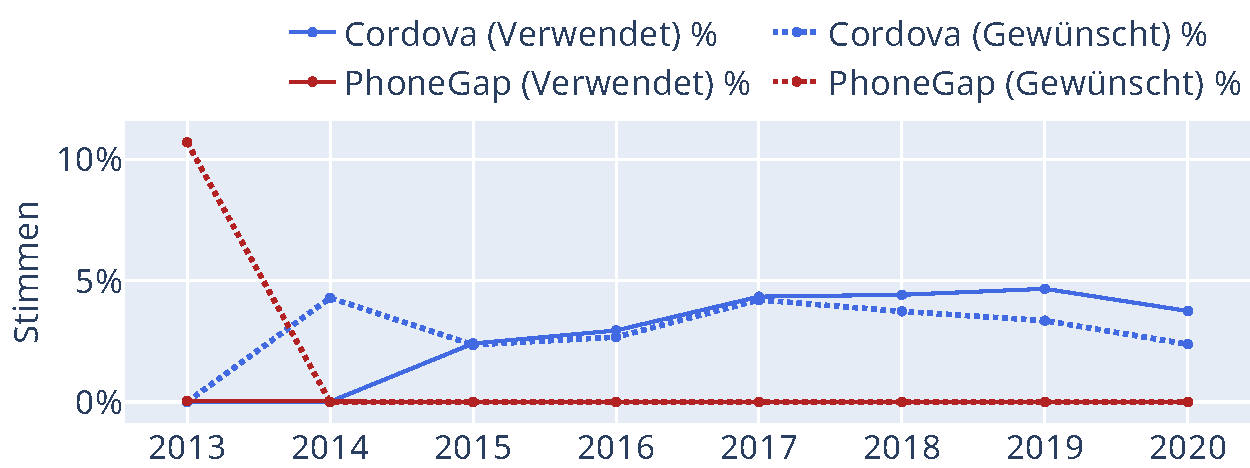
\includegraphics[width=1.0\textwidth]{Charts/Stack Overflow Umfrage/Cordova und PhoneGap Stimmen.pdf}
	\caption[Stimmen für Cordova und PhoneGap 2013 bis 2020]{Stimmen für Cordova und PhoneGap 2013 bis 2020, Quelle: Eigene Abbildung, Notebook: Charts/Stack Overflow Umfrage/Stack Overflow Umfrage.ipynb}
	\label{fig:CordovaUndPhoneGapStimmen}
\end{figure}
 
Am Beispiel von Adobe PhoneGap wird deutlich, wie wichtig es ist, auf eine Technologie zu setzen, die weit verbreitet ist. Im schlimmsten Fall wird die Technologie sogar vom Betreiber aufgrund zu geringer Nutzung komplett eingestellt, wie es bereits bei PhoneGap geschehen ist. Adobe gab am 11. August 2020 bekannt, dass die  Entwicklung an PhoneGap eingestellt wird und empfiehlt die Migration hin zu Apache Cordova.\footnote{Vgl. \cite{UpdateForCustomersUsingPhoneGapAndPhoneGapBuild}}

\subsubsection{Frameworks mit sinkender Relevanz}

Die Technologien Xamarin und Cordova zeigen bereits einen abfallenden Trend, wie in Abbildung \ref{fig:XamarinUndCordovaStimmen} ersichtlich ist. Im Fall von Xamarin gibt es immerhin mehr Entwickler, die sich wünschen, mit dem Framework zu arbeiten, als Entwickler, die tatsächlich mit Xamarin arbeiten. Cordova scheint in diesem Hinblick dagegen eher unbeliebt: es gibt mehr Entwickler, die mit Cordova arbeiten, als tatsächlich damit arbeiten wollen.

\begin{figure}[h]
	\centering
    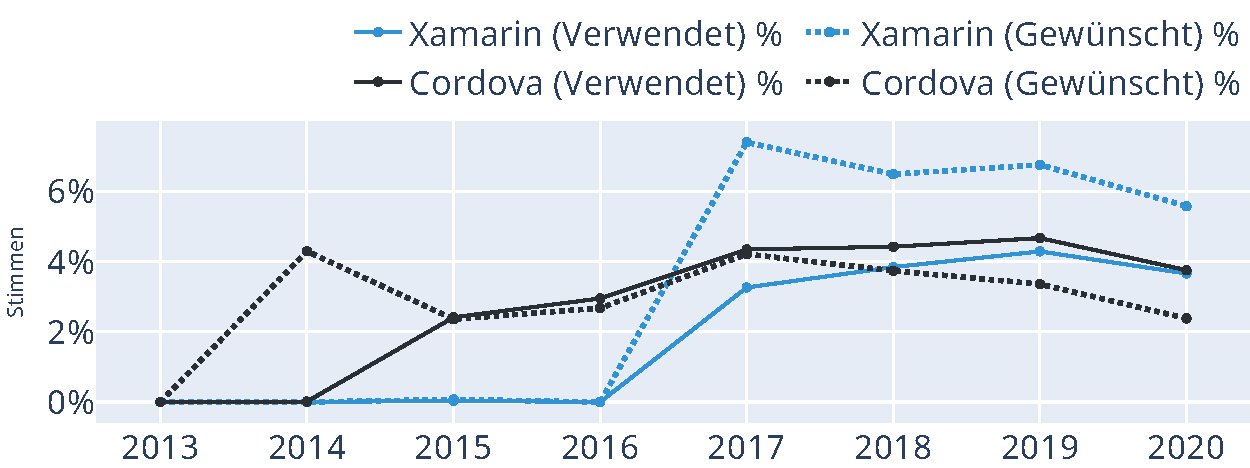
\includegraphics[width=1.0\textwidth]{Charts/Stack Overflow Umfrage/Xamarin und Cordova Stimmen.pdf}
	\caption[Stimmen für Xamarin und Cordova]{Stimmen für Xamarin und Cordova 2013 bis 2020, Quelle: Eigene Abbildung, Notebook: Charts/Stack Overflow Umfrage/Stack Overflow Umfrage.ipynb}
	\label{fig:XamarinUndCordovaStimmen}
\end{figure}

In Abbildung \ref{fig:SuchinteresseSinkendeUndSteigendeRelevanz} ist noch einmal zu sehen, dass Google Trends die Erkenntnisse aus der Stack Overflow Umfrage reflektiert und es wird auch sichtbar, welche beiden Technologien möglicherweise der Grund für den Rückgang von Xamarin und Cordova sind.

\begin{figure}[h]
	\centering
    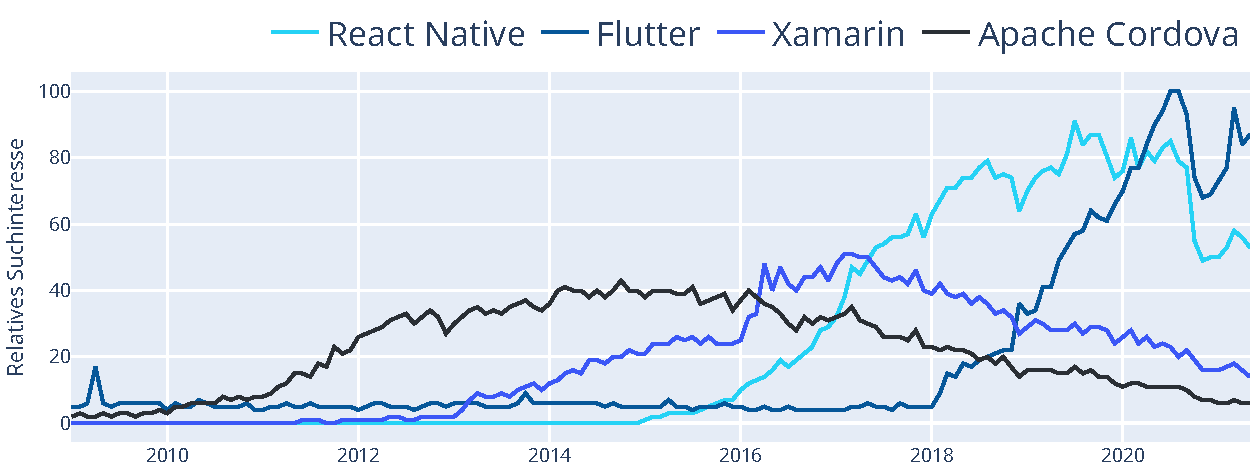
\includegraphics[width=1.0\textwidth]{Charts/Google Trends/Suchinteresse sinkende und steigende Relevanz.pdf}
	\caption[Suchinteresse sinkende und steigende Relevanz]{Suchinteresse sinkende und steigende Relevanz, Quelle: Eigene Abbildung, Notebook: Charts/Stack Overflow Umfrage/Stack Overflow Umfrage.ipynb}
	\label{fig:SuchinteresseSinkendeUndSteigendeRelevanz}
\end{figure}

\subsubsection{Frameworks mit steigender Relevanz}

Besser ist es, auf Technologien zu setzen, die noch einen steigenden Trend der Verbreitung und Beliebtheit zeigen. In Abbildung \ref{fig:ReactNativeUndFlutterStimmen} wird sichtbar, dass es sich dabei um Flutter und immerhin im Hinblick auf die Verbreitung auch für React Native handelt. Ungünstigerweise wird React Native in der Stack Overflow Umfrage erst seit 2018 als tatsächliches Framework abgefragt. Vorher erschien lediglich das Framework React, welches nicht für den Vergleich der Cross-PlatformFrameworks eignet, da es sich um ein reines Web-Framework handelt. Doch auch die Ergebnisse von Google Trends zeigen einen ähnlichen Verlauf für die Jahre 2019 und 2020 (Abb. \ref{fig:SuchinteresseSinkendeUndSteigendeRelevanz}).

\begin{figure}[h]
	\centering
    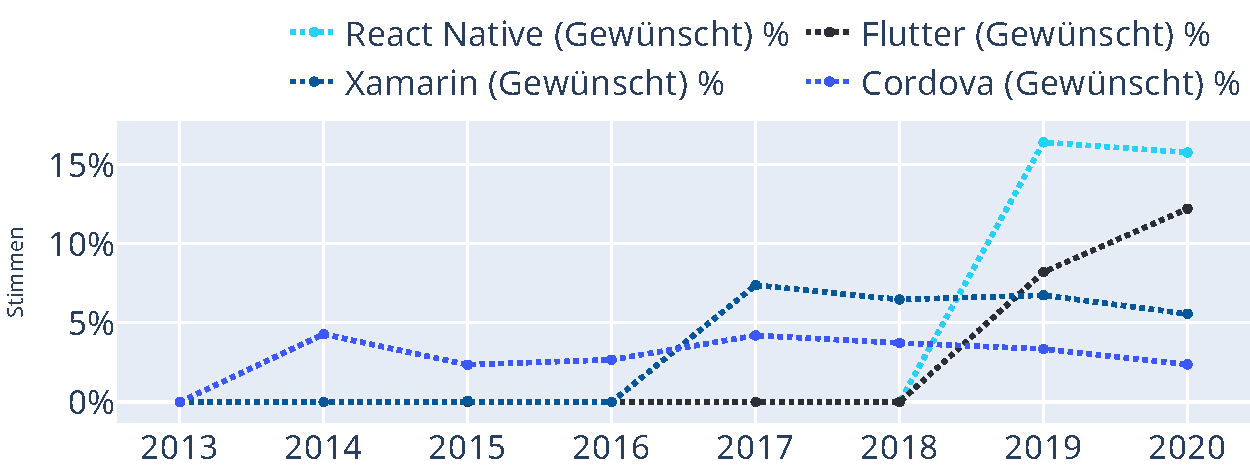
\includegraphics[width=1.0\textwidth]{Charts/Stack Overflow Umfrage/React Native und Flutter Stimmen.pdf}
	\caption[Stimmen für React Native und Flutter]{Stimmen für React Native und Flutter 2013 bis 2020, Quelle: Eigene Abbildung, Notebook: Charts/Stack Overflow Umfrage/Stack Overflow Umfrage.ipynb}
	\label{fig:ReactNativeUndFlutterStimmen}
\end{figure}

Im Vergleich von dem Jahr 2019 mit 2020 wird sichbar, dass die Zahl der Entwickler, die sich wünschen, mit React Native zu arbeiten, gesunken ist. Dennoch ist die Anzahl der Entwickler, die mit React Native arbeiten möchten noch weit höher, als die der Entwickler, die tatsächlich mit React Native arbeiten.

Es ist möglich, dass der abfallende Trend daran liegt, dass die Zahl der Entwickler, die mit Flutter arbeiten möchten im selben Jahr gestiegen ist. React Native hat im Vergleich zu Flutter jedoch noch immer mehr aktive Entwickler und die Tendenz ist steigend. Doch die Anzahl der aktiven Flutter Entwickler zeigt einen noch stärker steigenden Trend. So könnte es sein, dass die Zahl der Flutter Entwickler die der React Native Entwickler in einem der nächsten Jahre überholt. Im Such-Interesse hat sich diese Entwicklung bereits vollzogen (Abb. \ref{fig:SuchinteresseSinkendeUndSteigendeRelevanz}).

Nichtsdestotrotz scheinen beide Technologien als Kandidaten für einen detaillierteren Vergleich für dieses Projekt in Frage zu kommen. Im nächsten Kapitel soll evaluiert werden, welches Framework für die Entwicklung der Formular-Anwendung angemessener ist.






\subsection{Vergleich React Native und Flutter}

\subsubsection{Vergleich zweier minimaler Beispiele für Formulare und Validierung}


Es soll eine Formularanwendung mit komplexer Validierung im Rahmen dieser These erstellt werden. Es ist durchaus sinnvoll, die beiden Technologien anhand von  Beispielanwendungen, welche Formulare und die Validierung dieser  beinhalten,   zu vergleichen.  Deshalb soll nachfolgend  jeweils eine solche Beispielanwendung der jeweiligen Technologie gefunden werden. Die Anwendungen werden sich stark voneinander unterscheiden, weshalb sie im nächsten Schritt vereinfacht und aneinander angeglichen werden.  Anschließend wird ersichtlich werden, nach welchen Kriterien sich die Technologien im Hinblick auf die Entwicklung der Formularanwendung vergleichen lassen.

\paragraph{React Native}

React native stellt nur eine vergleichsweise geringe Anzahl von eigenen Komponenten zur Verfügung und zu diesen gehören keine, welche die Validierung von Formularen ermöglichen. Doch die im react.js Raum sehr bekannten Bibliotheken Formic, Redux Forms und React Hook Form sind alle drei kompatibel mit React Native.\footnote{Vgl. \cite{ReactNativeFormikDocs}}\footnote{Vgl. \cite{DoesReduxFormWorkWithReactNative}}\footnote{Vgl. \cite{ReactNativeReactHookFormGetStarted}}




Für die Formular-Anwendung ist die Validierung komplexer Bedingungen nötig. Die Formular-Validierungs-Bibliotheken bieten in der Regel Funktionen an, welche überprüfen, ob ein Feld gefüllt ist oder der Inhalt einem speziellen Muster entspricht – wie etwa einem regulären Ausdruck. Doch solche mitgelieferten Validierungs-Funktionen reichen nicht aus, um die Komplexität der Bedingungen abzubilden. Stattdessen müssen benutzerdefinierte Funktionen zum Einsatz kommen.

Keiner der drei oben genannten Validierungs-Bibliotheken ist in dieser Hinsicht limitiert. Sie alle bieten die Möglichkeit, eine JavaScript Funktion für die Validierung zu übergeben. Diese Funktion gibt einen Wahrheitswert zurück – wahr, wenn das Feld oder die Felder valide sind, falsch, falls nicht. In React Hook Form ist es die Funktion register, die ein Parameter-Objekt namens Register Options erhält, dessen Eigenschaft validate die JavaScript Funktion zugewiesen werden kann.\footnote{Vgl. \cite{RegisterReactHookFormAPI}}
In Redux Form ist es die Initialisierungs-Funktion reduxForm, die ein Konfigurations-Objekt mit dem Namen config erhält, in welchem die Eigenschaft ebenfalls validate heißt.\footnote{Vgl. \cite{ReduxFormReduxFormAPI}}
Auch in Formic ist der Bezeichner validate, und ist als Attribut in der Formic Komponente  zu finden.\footnote{Vgl. \cite{FormikComponentFormikDocsAPI}}


Es ist also absehbar, dass die Formular-Anwendung in React Native entwickelt werden kann.
Die nötigen Funktionen werden von den Bibliotheken bereitgestellt.
Einziger Nachteil hierbei ist, dass es sich um Drittanbieter Bibliotheken handelt, welche im Verlauf der Zeit an Beliebtheit gewinnen und verlieren können.
Möglicherweise geht die Beliebtheit einer der Bibliotheken mit der Zeit zurück, weshalb es weniger Kontributionen wie etwa neue Funktionalitäten oder Fehlerbehebungen, sowie Fragen und Antworten und Anleitungen zu diesen Bibliotheken geben wird, da die Entwickler sich für andere Bibliotheken entscheiden.
Die Wahl der Bibliothek kann also schwerwiegende Folgen wie Mangel an Dokumentation oder Limitationen im Vergleich zu anderen Bibliotheken mit sich bringen.
Eine Migration von der einen Bibliothek zu einer anderen könnte in Zukunft notwendig werden, wenn diese Limitationen während der Entwicklung auffallen. Aus dem Grund ist es in der Regel von Vorteil, wenn solche Funktionalitäten bereits im Kern der Frontend-Technologie integriert sind.
Der Fall, dass die Kern-Komponenten an Relevanz verlieren und empfohlen wird, auf externe Bibliotheken zuzugreifen, ist zwar nicht ausgeschlossen, geschieht aber im Wesentlichen seltener.



















\paragraph{Flutter}
Die Flutter Dokumentation stellt in ihrer cookbook Sektion ein Beispiel einer minimalistischen Formularanwendung mit Validierung bereit.\footnote{Vgl. \cite{BuildAFormWithValidation}} Das Rezept ist Teil einer Serie von insgesamt fünf Anleitungen, welche Formulare in Flutter behandeln.\footnote{Vgl. \cite{FormsFlutter}}

\subsubsection{Automatisiertes Testen}

\paragraph{Automatisierte Tests in React Native} Die React Native Dokumentation führt genau eine Seite mit einem Überblick über die unterschiedlichen Testarten. Dabei wird das Konzept von Unit Tests, Mocking, Integrations Tests, Komponenten Tests und Snapshot Tests kurz erläutert, jedoch ohne ein Beispiel zu geben oder zu verlinken. Vier Quellcodeschnipsel sind auf der Seite zu finden: Ein Schnipsel zeigt den minimalen Aufbau eines Tests, zwei weitere Schnipsel veranschaulichen beispielhaft, wie Nutzerinteraktionen getestet werden können und Letzteres zeigt die textuelle Repräsentation der Ausgabe einer Komponente, die für einen Snapshottest verwendet wird. Weiterhin wird auf die Jest API Dokumentation verwiesen, sowie auf ein Beispiel für einen Snapshot Test in der Jest Dokumentation.\footnoteL{\url{https://jestjs.io/docs/snapshot-testing}}

Um die notwendigen Anleitungen für das Erstellen der jeweiligen Tests ausfindig zu machen, ist es notwendig, die Dokumentation von React Native zu verlassen.

Die Dokumentation von Jest enthält mehr Details zum Einsatz der Testbibliothek, welches für mehrere auf Javascript basierende Frontend Frameworks kompatibel ist\footnoteL{\url{https://jestjs.io/docs/getting-started}}. Somit muss zum Erstellen der Unit-Tests immerhin nur dieses Framework studiert werden.

Zum Entwickeln von Tests von React Native Komponenten wird unter anderem auf die Bibliothek React Native Testing Library verwiesen. Anders als der Name vermuten lässt, handelt es sich nicht um eine von React Native bereitgestellte Bibliothek. Im Unterschied zur React Testing Library, von der sie inspiriert ist, läuft sie  ebenso  wie React Native selbst nicht in einer Browser-Umgebung.\footnote{Vgl. \cite{NativeTestingLibraryIntroduction}} Herausgegeben wird die React Native Testing Library vom Drittanbieter Callstack - ein Partner im React Native Ökosystem.\footnote{Vgl. \cite{TheReactNativeEcosystem}}

Sie verwendet im Hintergrund den React Test Renderer\footnoteL{\url{https://reactjs.org/docs/test-renderer.html}}, welcher wiederum vom React Team angeboten wird und auch zum Testen von react.js Anwendungen geeignet ist. Der React Test Renderer wird ebenfalls empfohlen, um Komponententests zu kreieren, die keine React Native spezifischen Funktionalitäten nutzen.

Um Integrationstests zu entwickeln - welche die Applikation auf einem physischen Gerät oder auf einem Emulator testen - wird auf zwei weitere Drittanbieter-Bibliotheken verlinkt: Appium\footnoteL{\url{http://appium.io/}} und Detox\footnoteL{\url{https://github.com/wix/detox/}}. Es wird darauf hingewiesen, dass Detox speziell für die Entwicklung von React Native Integrationstests entwickelt wurde. Appium wird lediglich als ein weiteres bekanntes Werkzeug erwähnt. 

Es lässt sich damit zusammenfassen, dass der Aufwand der Einarbeitung für automatisiertes Testen in React Native vergleichsweise hoch ist. Die Dokumentation ist auf die Seiten der jeweiligen Anbieter verteilt. Der Entwickler muss sich den Überblick selbst verschaffen und zusätzlich die für das Framework React Native relevanten Inhalte identifizieren. Notwendig ist auch das Erlernen von mehreren APIs um alle Testarten abzudecken. Für einen Anfänger kommt erschwerend hinzu, dass eine Entscheidung für die eine oder andere Bibliothek notwendig wird. Um diese Entscheidung treffen zu können, ist eine Auseinandersetzung mit den Vor- und Nachteilen der Technologien im Vorfeld vom Entwickler zu leisten.

\paragraph{Automatisierte Tests in Flutter} Die Flutter Dokumentation erklärt sehr umfangreich auf 11 Unterseiten die unterschiedlichen Testarten mit Quellcodebeispielen und verlinkt für jede Testart eine bis mehrere detaillierte Schritt-für-Schritt-Anleitungen, wie ein solcher Test erstellt wird.

Eine Seite erklärt den Unterschied zwischen Unit Test, Widget Test und Integrationstest\footnoteL{\url{https://flutter.dev/docs/testing}}. Eine weitere Seite erklärt Integrationstests in mehr Detail\footnoteL{\url{https://flutter.dev/docs/testing/integration-tests}}. 

Ein sogenanntes Codelab führt durch die Erstellung einer minimalistischen App und zwei Unit-, fünf Widget- und zwei Integrationstest für diese App\footnoteL{\url{https://codelabs.developers.google.com/codelabs/flutter-app-testing}}

Im sogenannten Kochbuch tauchen folgende Rezepte auf:

\begin{itemize}
    \item 2 Rezepte für Unit Tests
    \begin{itemize} 
       \item eine grundlegende Anleitung zum Erstellen von Unit-Tests \footnoteL{\url{https://flutter.dev/docs/cookbook/testing/unit/introduction}}
       \item Eine weitere Anleitung zum Nutzen von mocks in Unit Test mithilfe der Bibliothek mockito \footnoteL{\url{https://flutter.dev/docs/cookbook/testing/unit/mocking}}
    \end{itemize}
    \item 3 Rezepte für Widget Tests
    \begin{itemize} 
        \item Eine grundlegende Anleitung zum Erstellen von Widget Test \footnoteL{\url{https://flutter.dev/docs/cookbook/testing/widget/introduction}}
        \item Ein Rezept mit detaillierteren Beispielen zum Finden von widgets  zur Laufzeit eines Widget Tests \footnoteL{\url{https://flutter.dev/docs/cookbook/testing/widget/finders}}
        \item Ein Rezept zum Testen von Nutzerverhalten wie dem Tab, dem Drag und dem eingeben von Text \footnoteL{\url{https://flutter.dev/docs/cookbook/testing/widget/tap-drag}}
     \end{itemize}
    \item 3 Rezepte für Integrationstests
    \begin{itemize} 
        \item Eine grundlegende Anleitung zum Erstellen eines Integrationstest \footnoteL{\url{https://flutter.dev/docs/cookbook/testing/integration/introduction}}
        \item eine Anleitung zum simulieren von scrollen in der Anwendung während der Laufzeit eines Integrationstest \footnoteL{\url{https://flutter.dev/docs/cookbook/testing/integration/scrolling}}
        \item eine Anleitung zum Performance Profiling \footnoteL{\url{https://flutter.dev/docs/cookbook/testing/integration/profiling}}
     \end{itemize}
\end{itemize}

Zusammengefasst: Der Aufwand der Einarbeitung in das Testen in Flutter ist gering. Alle Werkzeuge werden vom Dart- und Flutter-Team bereitgestellt. Die Dokumentation ist umfangreich, folgt jedoch einem roten Faden. Eine Übersichtsseite fasst die Kerninformationen zusammen und verweist auf die jeweiligen  Seiten für detailliertere Informationen und Übungen.

Wunsch
\begin{itemize}
	\item Alle Komponenten wiederverwendbar wie etwa Selection Caard nicht nur für Choices
	\item 
\end{itemize}

\begin{itemize}
	\item Strategy Entwurfsmuster für compute choice von viewModelType weil viewmodel nötig ist für nested formular
	\item 
\end{itemize}

\section{Model View ViewModel}

\subsection{Model}
\subsection{View}
\subsection{ViewModel}


\section{Selection Card}

\subsection{Strategie Entwurfsmuster}
\subsubsection{On Select On Deselect Strategie}
\subsubsection{Compute Choice Strategie}


\subsection{Single Selection}
\subsubsection{View Model}
\paragraph{Choice}
\subsubsection{View}
\subsubsection{Model}

\subsection{Multi Selection Selection}
\subsubsection{View Model}
\paragraph{BuiltSet}
\subsubsection{View}
\subsubsection{Model}

\subsection{Nested Selection}
\subsubsection{View Model}
\paragraph{BuiltMap}
\paragraph{Nested View Model}
\paragraph{Convertierung View Model und Model}
\paragraph{Nested View Strategie}
\subsubsection{Extensions Methods VS Compute Choice from Selection Model}

\subsubsection{View}
\subsubsection{Model}

\section{Doktorarbeit}
\subsection{Condtions}
\subsubsection{And}
\paragraph{Check}
\paragraph{Finde invalide oder fehlende Auswahl}

\subsubsection{Or}
\paragraph{Check}
\paragraph{Finde invalide oder fehlende Auswahl}

\subsubsection{In}
\paragraph{Check}
\paragraph{Finde invalide oder fehlende Auswahl}


\subsubsection{NotIn}
\subsubsection{Exclusive}
\subsubsection{Always Met}


\subsection{Fluent API} 


\subsection{Chart}
\subsubsection{Generiere Chart automatisch und Rekursiv aus Datenstrucktur}
\subsubsection{Zeichne invalide oder fehlende Auswahl}

\subsubsection{conditions_chart.dart}

Gespräch mit Daniel über Doktorarbeit
math bibliotheken

ki

viel detailiertere beschreibungen ausführungen nötig
mehr recherche nötig



fachwissen anwenden
fachwissen abstrahieren
	transfer

	weg der transferleistung beschreiben können


wenn übertragung der abstrakten in ein neues feld passiert
	die methoden neu
	das was dabei passiert neu ist
		die methoden neu ist

\begin{appendix} 
  \section*{Anhang} 
  \addcontentsline{toc}{section}{Anhang}%\addtocontents{toc}{\vfill}
  \renewcommand{\thesubsection}{\Alph{subsection}}
 
  \subsection{Technologiewahl Anhang} 

\subsubsection{Stimmen verwendeter Frameworks} 

\begin{figure}[H]
	\centering
    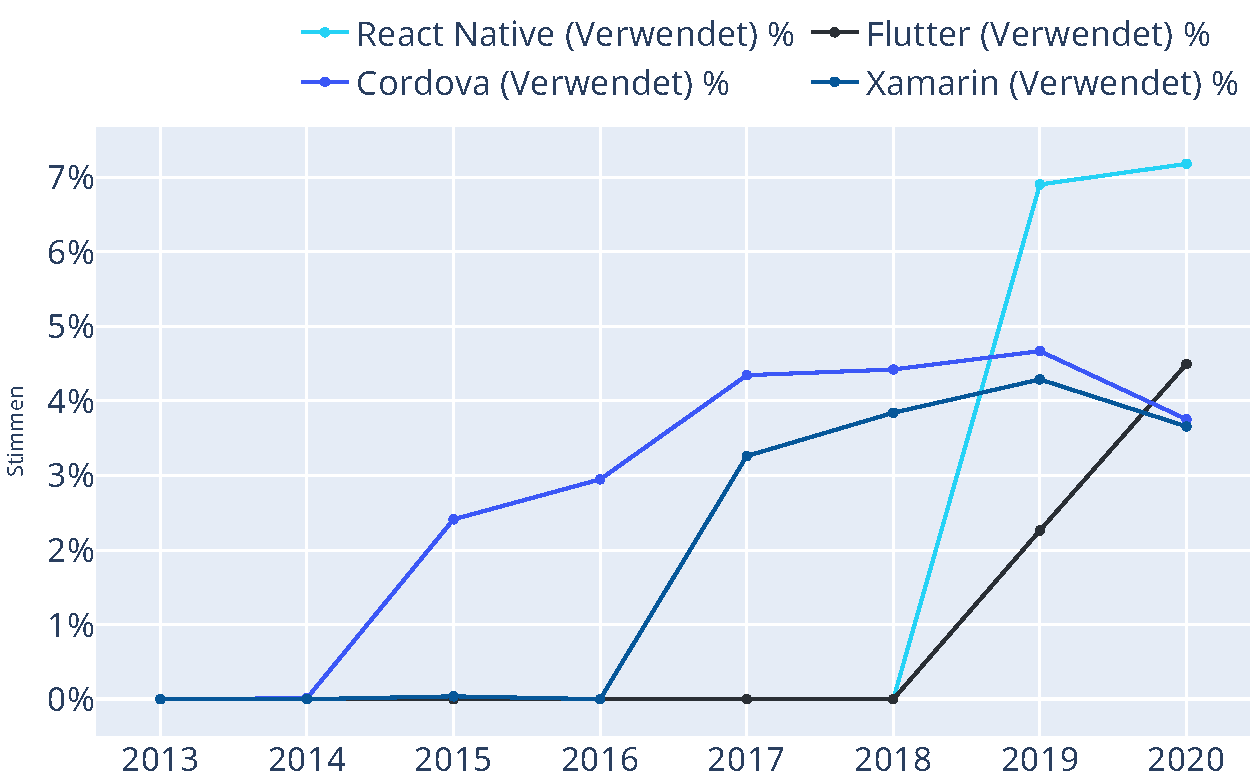
\includegraphics[width=1.0\textwidth]{Charts/Stack Overflow Umfrage/Stimmen verwendeter Frameworks.pdf}
	\caption[Stimmen verwendeter Frameworks]{Stimmen verwendeter Frameworks, Quelle: Eigene Abbildung, Notebook: Charts/Stack Overflow Umfrage/Stack Overflow Umfrage.ipynb}
	\label{fig:StimmenVerwendeter Frameworks}
\end{figure}


\subsubsection{Stimmen gewünschter Frameworks} 

\begin{figure}[H]
	\centering
    \includegraphics[width=1.0\textwidth]{Charts/Stack Overflow Umfrage/Stimmen gewünschter Frameworks.pdf}
	\caption[Stimmen gewünschter Frameworks]{Stimmen gewünschter Frameworks, Quelle: Eigene Abbildung, Notebook: Charts/Stack Overflow Umfrage/Stack Overflow Umfrage.ipynb}
	\label{fig:StimmenGewuenschterFrameworks}
\end{figure}





\subsection{Vergleich React Native und Flutter Anhang} 


\begin{listing}[H]
	\label{lst:quelltext1}

    \begin{minted}[
        linenos, % Quelltextzeilen anzeigen
        numbersep=5pt, %Abstand
        firstnumber=1,
        frame=lines,
        fontsize=\small,
        framesep=2mm,
		tabsize=4,
		breaklines,
		breakafter=_@|
        ]{dart}
import 'package:flutter/material.dart';
import 'input.dart';

void main() => runApp(MyApp());

class MyApp extends StatelessWidget {
  @override
  Widget build(BuildContext context) => MaterialApp(
		home: Scaffold(
		  body: MyCustomForm(),
		),
	  );
}

final emailPattern = new RegExp(
    r'^(([^<>()\[\]\\.,;:\s@\enquote{]+(\.[^<>()\[\]\\.,;:\s@} ]+)*)|(\enquote{.+} ))@((\[[0-9]{1,3}\.[0-9]{1,3}\.[0-9]{1,3}\.[0-9]{1,3}\])|(([a-zA-Z\-0-9]+\.)+[a-zA-Z]{2,}))$');

class MyCustomForm extends StatefulWidget {
  @override
  MyCustomFormState createState() => MyCustomFormState();
}

class MyCustomFormState extends State<MyCustomForm> {
  final _formKey = GlobalKey<FormState>();

  @override
  Widget build(BuildContext context) => Form(
		key: _formKey,
		child: Padding(
		  padding: const EdgeInsets.all(8.0),
		  child: Column(
			children: [
			  Input(label: \enquote{Name} ),
			  Input(
				  label: \enquote{Email} ,
				  validator: (value) {
					if (value == null || !emailPattern.hasMatch(value)) {
					  return 'Invalid Email Format';
					}
					return null;
				  }),
			  Input(label: \enquote{Password} ),
			  Padding(
				padding: const EdgeInsets.symmetric(vertical: 16.0),
				child: ElevatedButton(
				  onPressed: () {
					if (_formKey.currentState!.validate()) {
					  ScaffoldMessenger.of(context).showSnackBar(
						  SnackBar(content: Text('Processing Data')));
					}
				  },
				  child: Text('Submit'),
				),
			  ),
			],
		  ),
		),
	  );
}
		
    \end{minted}

    \caption[main.dart]{main.dart Datei}
\end{listing}


\begin{listing}[H]
	\label{lst:quelltext2}

    \begin{minted}[
        linenos, % Quelltextzeilen anzeigen
        numbersep=5pt, %Abstand
        firstnumber=1,
        frame=lines,
        fontsize=\small,
        framesep=2mm,
		tabsize=4,
		breaklines,
		breakafter=_@|
        ]{javascript}
export default {
	name: {required: {value: true, message: 'Name is required'}},
	email: {
	  required: {value: true, message: 'Email is required'},
	  pattern: {
		value: /^(([^<>()\[\]\\.,;:\s@\enquote{]+(\.[^<>()\[\]\\.,;:\s@} ]+)*)|(\enquote{.+} ))@((\[[0-9]{1,3}\.[0-9]{1,3}\.[0-9]{1,3}\.[0-9]{1,3}\])|(([a-zA-Z\-0-9]+\.)+[a-zA-Z]{2,}))$/,
		message: 'Invalid Email Format',
	  },
	},
	password: {
	  required: {value: true, message: 'Password is required'},
	},
  };
    \end{minted}

    \caption[validation.tsx]{validation.tsx Datei}
\end{listing}


\begin{listing}[H]
	\label{lst:quelltext3}

    \begin{minted}[
        linenos, % Quelltextzeilen anzeigen
        numbersep=5pt, %Abstand
        firstnumber=1,
        frame=lines,
        fontsize=\small,
        framesep=2mm,
		tabsize=4,
		breaklines,
		breakafter=_@|
        ]{dart}
final emailPattern = new RegExp(
	r'^(([^<>()\[\]\\.,;:\s@\enquote{]+(\.[^<>()\[\]\\.,;:\s@} ]+)*)|(\enquote{.+} ))@((\[[0-9]{1,3}\.[0-9]{1,3}\.[0-9]{1,3}\.[0-9]{1,3}\])|(([a-zA-Z\-0-9]+\.)+[a-zA-Z]{2,}))$');

validateEmail(value) {
  if (value == null || !emailPattern.hasMatch(value))
	return 'Invalid Email Format';
  else
	return null;
}

validateNotEmpty(String label, value) {
  if (value == null || value.isEmpty)
	return '$label is required';
  else
	return null;
}		
    \end{minted}

    \caption[validation.dart]{validation.dart Datei}
\end{listing}


\begin{listing}[H]
	\label{lst:quelltext4}

    \begin{minted}[
        linenos, % Quelltextzeilen anzeigen
        numbersep=5pt, %Abstand
        firstnumber=1,
        frame=lines,
        fontsize=\small,
        framesep=2mm,
		tabsize=4,
		breaklines,
		breakafter=_@|
        ]{dart}
import 'package:example_form_app/validation.dart';
import 'package:flutter/material.dart';

class Input extends StatelessWidget {
  final String label;
  final FormFieldValidator<String>? validator;

  const Input({required this.label, this.validator});

  @override
  Widget build(BuildContext context) => TextFormField(
	  decoration: InputDecoration(labelText: label),
	  validator: validator ?? (value) => validateNotEmpty(label, value));
}
    \end{minted}

    \caption[input.dart]{input.dart Datei}
\end{listing}













\begin{listing}[H]
	\label{lst:quelltext5}

    \begin{minted}[
        linenos, % Quelltextzeilen anzeigen
        numbersep=5pt, %Abstand
        firstnumber=1,
        frame=lines,
        fontsize=\small,
        framesep=2mm,
		tabsize=4,
		breaklines,
		breakafter=_@|
        ]{javascript}
import * as React from 'react';
import { TextInput, KeyboardAvoidingView, findNodeHandle } from 'react-native';
import { ValidationOptions, FieldError } from 'react-hook-form';

interface ValidationMap {
  [key: string]: ValidationOptions;
}

interface ErrorMap {
  [key: string]: FieldError | undefined;
}

interface Props {
  children: JSX.Element | JSX.Element[];
  register: (
    field: { name: string },
    validation?: ValidationOptions
  ) => void;
  errors: ErrorMap;
  validation: ValidationMap;
  setValue: (name: string, value: string, validate?: boolean) => void;
}
\end{minted}


\caption[Form.tsx]{Form.tsx Datei}
\end{listing}

\begin{listing}[H]
	\label{lst:quelltext6}
    \inputminted[lastline=23, linenos, numbersep=5pt, firstnumber=1, frame=lines, fontsize=\small, framesep=2mm, tabsize=4, breaklines, breakafter=_@|]
    {typescript}
    {source_code/flutter_vs_react_native/react_native/example_form_app/form-in-react-native-the-right-way/components/Form.tsx}
\caption[Form.tsx]{Form.tsx Datei}
\end{listing}
 
\begin{listing}[H]
	\label{lst:quelltext7}
    \inputminted[firstline=24, linenos, numbersep=5pt, firstnumber=24, frame=lines, fontsize=\small, framesep=2mm, tabsize=4, breaklines, breakafter=_@|]
    {typescript}
    {source_code/flutter_vs_react_native/react_native/example_form_app/form-in-react-native-the-right-way/components/Form.tsx}
\caption[Form.tsx]{Form.tsx Datei}
\end{listing}




\begin{listing}[H]
	\label{lst:quelltext8}
    \begin{minted}[
        linenos, % Quelltextzeilen anzeigen
        numbersep=5pt, %Abstand
        firstnumber=1,
        frame=lines,
        fontsize=\small,
        framesep=2mm,
		tabsize=4,
		breaklines,
		breakafter=_@|
        ]{javascript}
import * as React from 'react';
import {
  View,
  TextInput,
  Text,
  StyleSheet,
  ViewStyle,
  TextStyle,
  TextInputProps,
} from 'react-native';
import { FieldError } from 'react-hook-form';
interface Props extends TextInputProps {
  name: string;
  label?: string;
  labelStyle?: TextStyle;
  error?: FieldError | undefined;
}

export default React.forwardRef<any, Props>(
  (props, ref): React.ReactElement => {
	const { label, labelStyle, error, ...inputProps } = props;

	return (
	  <View style={styles.container}>
		{label && <Text style={[styles.label, labelStyle]}>{label}</Text>}
		<TextInput
		  autoCapitalize=\enquote{none}
		  ref={ref}
		  style={[styles.input, { borderColor: error ? '#fc6d47' : '#c0cbd3' }]}
		  {...inputProps}
		/>
		<Text style={styles.textError}>{error && error.message}</Text>
	  </View>
	);
  }
);

const styles = StyleSheet.create({
  container: {
	marginVertical: 8,
  },
  input: {
	borderWidth: 1,
	paddingLeft: 5,
  },
  label: {
	paddingVertical: 5,
  },
  textError: {
	color: '#fc6d47',
  },
});	
\end{minted}


\caption[Input.tsx]{Input.tsx Datei}
\end{listing}


 

\begin{listing}[H]
	\label{lst:quelltext9}

    \begin{minted}[
        linenos, % Quelltextzeilen anzeigen
        numbersep=5pt, %Abstand
        firstnumber=1,
        frame=lines,
        fontsize=\small,
        framesep=2mm,
		tabsize=4,
		breaklines,
		breakafter=_@|
        ]{javascript}
import * as React from 'react';
import {
  Text,
  View,
  StyleSheet,
  Button,
  Alert,
  ScrollView,
} from 'react-native';

import { useForm } from 'react-hook-form';

import Input from './components/Input';
import Form from './components/Form';
import validation from './validation';

type FormData = {
  name: string;
  email: string;
  password: string;
};

export default () => {
  const { handleSubmit, register, setValue, errors } = useForm<FormData>();

  const onSubmit = (data: FormData) => {
	Alert.alert('data', JSON.stringify(data));
  };

  return (
	  <View style={styles.formContainer}>
		<Form {...{ register, setValue, validation, errors }}>
		  <Input name=\enquote{name} label=\enquote{Name } />
		  <Input name=\enquote{email} label=\enquote{Email} />
		  <Input name=\enquote{password} label=\enquote{Password} secureTextEntry={true} />
		  <Button title=\enquote{Submit} onPress={handleSubmit(onSubmit)} />
		</Form>
	  </View>
  );
};

const styles = StyleSheet.create({
  formContainer: {
	padding: 8,
	flex: 1,
  }
});		
\end{minted}


\caption[App.tsx]{App.tsx Datei}
\end{listing}


\end{appendix} 

\printbibliography{}

\include{content/appendix/appendix} 

% \include{content/misc/eidesstattliche_erklaerung}
% \section*{Eidesstattliche Erklärung}

\addcontentsline{toc}{section}{Eidesstattliche Erklärung}

\vspace{10mm}

Ich versichere, dass ich die vorstehende Arbeit selbständig angefertigt und mich fremder 
Hilfe nicht bedient habe. Alle Stellen, die wörtlich oder sinngemäß veröffentlichtem oder 
nicht veröffentlichtem Schrifttum entnommen sind, habe ich als solche kenntlich gemacht.

\vspace{10mm}

Wernigerode, den 16.11.2020 

\begin{flushright}
    $\overline{~~~~~~~~~\mbox{Alexander Johr}~~~~~~~~~}$
\end{flushright}

\end{document}
